\chapter{Conclusion}

The Daya Bay Reactor Neutrino Experiment is a precision measurement of $\theta_{13}$ designed to measure $\sin^22\theta_{13}$ with sensitivity $<0.01$ at 90\% confidence level. In 2012 Daya Bay discovered that $\theta_{13}$ is nonzero with 5.2$\sigma$ and $\sin^22\theta_{13}=0.092\pm0.016(\text{stat.})\pm0.005(\text{syst.})$~\cite{dayabay2012_1}. The fast neutron background constitutes one of the five backgrounds in $\theta_{13}$ measurement. Therefore understanding the neutron yield induced by cosmic ray muons is important.

In this study we make a well-defined cylindrical fiducial volume of fixed radius around each muon track. Only neutrons captured in the fiducial volume is counted. We use the lateral distribution of the neutron captured position to correct for the inefficiency due to the neutrons leaking out of the fiducial volume.

The muon tracks are reconstructed by connecting the RPC and OWS reconstructed points. The RPC positions are reconstructed by the centroids of the fired $x$ and $y$ strips with a resolution of $\sim 7$ cm. The OWS positions are reconstructed by the charge-weighted mean of the positions of fired PMTs whose resolution is $\sim 60$ cm. The neutron captured positions are reconstructed by charge-weighted mean corrected by Monte Carlo simulation with a resolution of $\sim 20$ cm. The resolutions of the reconstruction algorithms are used for estimating errors in the neutron yield determination. Details in constructing the fiducial volumes can be found in Appendix~\ref{app:a}.

The neutron yield produced by muons in liquid scintillator was measured at Daya Bay to be about $10^{-4} cm^2/\mu/g$. These results are in agreement with previous measurements~\cite{Agafonova2013}. Figure~\ref{fig:neutron_yield_chap8} shows the results obtained in this study on top of the previous measurements.
\begin{figure}
	\centering
	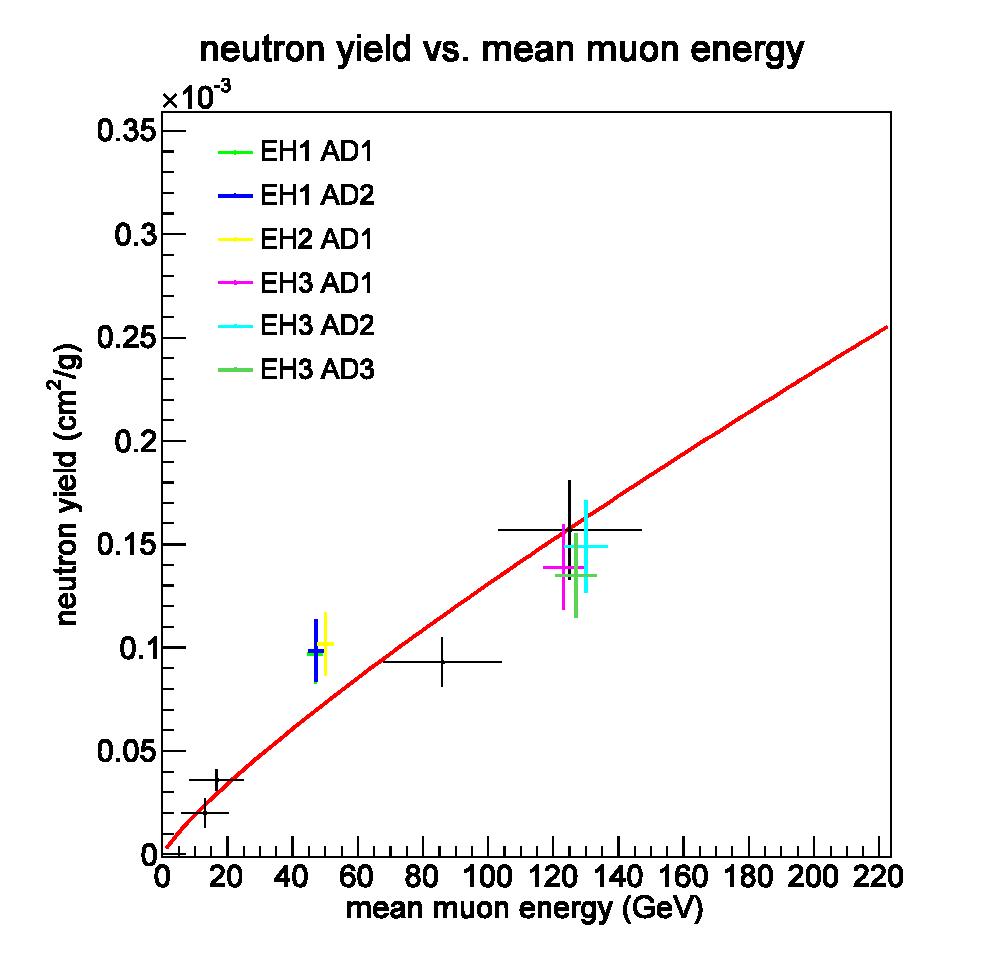
\includegraphics[width=0.7\textwidth]{figures/chap8/neutron_yield.eps}
	\caption[Neutron yield as a function of the mean muon energy. Colored points are results in this study. Black dots are from previous measurements. The red curve is the power law fit to the black dots.]{Neutron yield as a function of the mean muon energy. Colored points are results in this study. Black dots are from previous measurements~\cite{Agafonova2013}. The red curve is the power law fit to the black dots.}
	\label{fig:neutron_yield_chap8}
\end{figure}
We also found evidence for additional energy deposition in neutron events.


%\clearpage % start a new page for references